\newcommand{\TODO}[1]{{\color{red}\textbf{TODO} #1}}

% TEMPLATE for Usenix papers, specifically to meet requirements of
%  USENIX '05
% originally a template for producing IEEE-format articles using LaTeX.
%   written by Matthew Ward, CS Department, Worcester Polytechnic Institute.
% adapted by David Beazley for his excellent SWIG paper in Proceedings,
%   Tcl 96
% turned into a smartass generic template by De Clarke, with thanks to
%   both the above pioneers
% use at your own risk.  Complaints to /dev/null.
% make it two column with no page numbering, default is 10 point

% Munged by Fred Douglis <douglis@research.att.com> 10/97 to separate
% the .sty file from the LaTeX source template, so that people can
% more easily include the .sty file into an existing document.  Also
% changed to more closely follow the style guidelines as represented
% by the Word sample file. 

% Note that since 2010, USENIX does not require endnotes. If you want
% foot of page notes, don't include the endnotes package in the 
% usepackage command, below.

% This version uses the latex2e styles, not the very ancient 2.09 stuff.
\documentclass[letterpaper,twocolumn,10pt]{article}
\usepackage{usenix2019,epsfig,endnotes}
\usepackage{color}
\usepackage{pifont}
\usepackage{hyperref}
\usepackage{subcaption}
\usepackage{listings}
\lstset{language=c,
   basicstyle=\small\ttfamily,
   keywordstyle=\color{black}\bfseries\underbar,
   numbers=none,
   numberstyle=\tiny,
   frame=single}

\begin{document}

%don't want date printed
\date{}

%make title bold and 14 pt font (Latex default is non-bold, 16 pt)
\title{\Large \bf Flightplan: dataplane disaggregation and coordination for in-network computing}

%for single author (just remove % characters)
\author{UPenn DCOMP}

\maketitle

% Use the following at camera-ready time to suppress page numbers.
% Comment it out when you first submit the paper for review.
\thispagestyle{empty}

\subsection*{Abstract}
Increased dataplane programmability is enabling new in-network services which
in turn benefit applications running on the network. But the interlinked
dataplanes forming a network are currently programmed disjointly as independent
entities.  Moreover these dataplanes are typically heterogeneous and offer
different trade-offs between performance and programmability.
We argue that in-network programmability needs a more cohesive
programming approach that extends across dataplanes to better leverage
network programmability and target heterogeneity, and improve
performance and utilisation.

We present Flightplan, a new dataplane programming approach that automatically
splits a \emph{single} dataplane program into a distributed system running on
different interconnected dataplanes.
Flightplan relies on a new, portable meta-programming construct to
delimit dataplane subprograms, and it simplifies the writing and
debugging of in-network programs through automated code generation.

We implement a Flightplan prototype for P4 and evaluate it using
a new suite of network functions on diverse hardware targets.
We find that dataplane disaggregation enables run-time tuning for
better performance and availability, and better utilisation of
heterogeneous network element resources.


\section{Introduction}
Network programmability has been inching from the edge of datacenter networks inwards
towards the core, as the dataplanes of higher-bandwidth and higher-radix
network elements become increasingly programmable. While there remains a broad
scope for using CPUs for network and middlebox programming~\cite{Fall:2011:REG:1945023.1945037,Laufer:2016:CEN:3027947.3027951,Bezahaf:2013:FFP:2535828.2535836,196178,Ballani:2015:EEN:2829988.2787493},
the use of hardware targets such as programmable ASICs, FPGAs, and
NPUs is transforming the capabilities of the network itself.

In particular, more computations can be pushed into the network
without sacrificing throughput and latency.  These computations
include more sophisticated network
logic~\cite{Giesen:2018:ICR:3229591.3229595} as well as application
logic~\cite{Jin:2017:NBK:3132747.3132764}, and precipitate a shift in
the conventional thinking about which functions are usually implemented
in the network, and which are left to edge
hosts~\cite{Saltzer:1984:EAS:357401.357402}.

\begin{figure}[t]
\centering
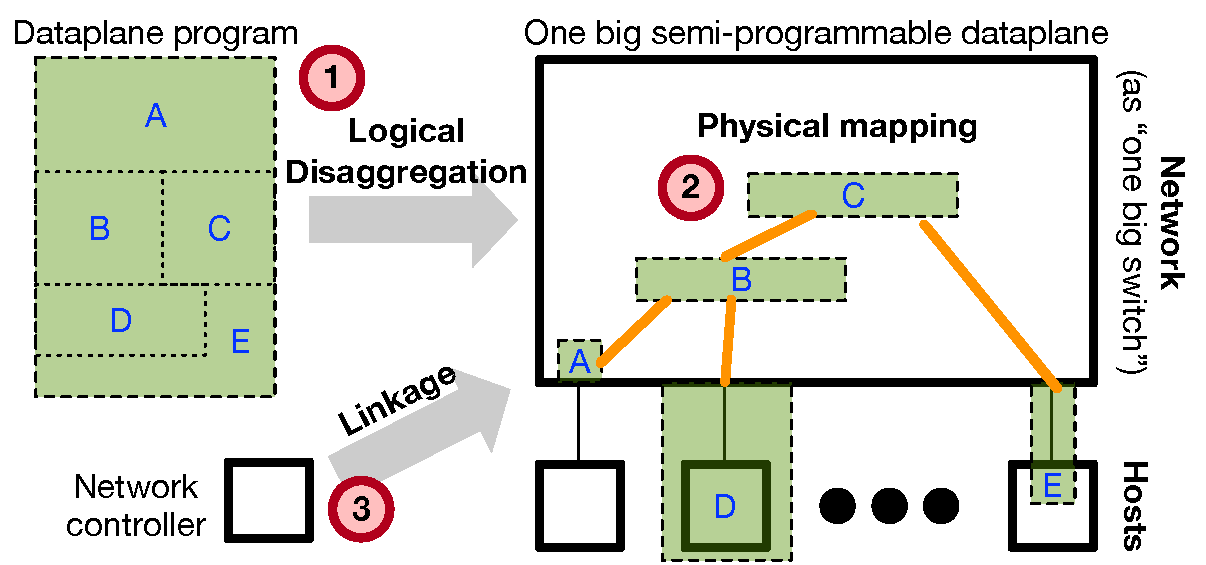
\includegraphics[width=0.5\textwidth]{overview.pdf}
\caption{\label{fig:overview}In this illustration a program is split into 5 logical parts, {\sf\color{blue} A}-{\sf\color{blue} E}.
{\color{red}\ding{192}}~A program is annotated with logical delimiters, which Flightplan uses to split the program into complementary parts. Flightplan generates coordination and linkage code between these parts, which the network controller can configure at runtime.
{\color{red}\ding{193}}~Each split of the original program is mapped to a physical device. In this illustration,
 {\sf\color{blue} A} is a ToR switch,
 {\sf\color{blue} B} and {\sf\color{blue} C} are aggregation or core switches,
 {\sf\color{blue} D} is a CPU-run packet processor, and
 {\sf\color{blue} E} is an NPU.
{\color{red}\ding{194}}~The network controller can alter the program's linkage at runtime, to use different hardware targets, mitigate faults, or balance load.
}
\end{figure}

\begin{figure*}[t!]
\centering
\begin{subfigure}[t]{0.5\textwidth}
\centering
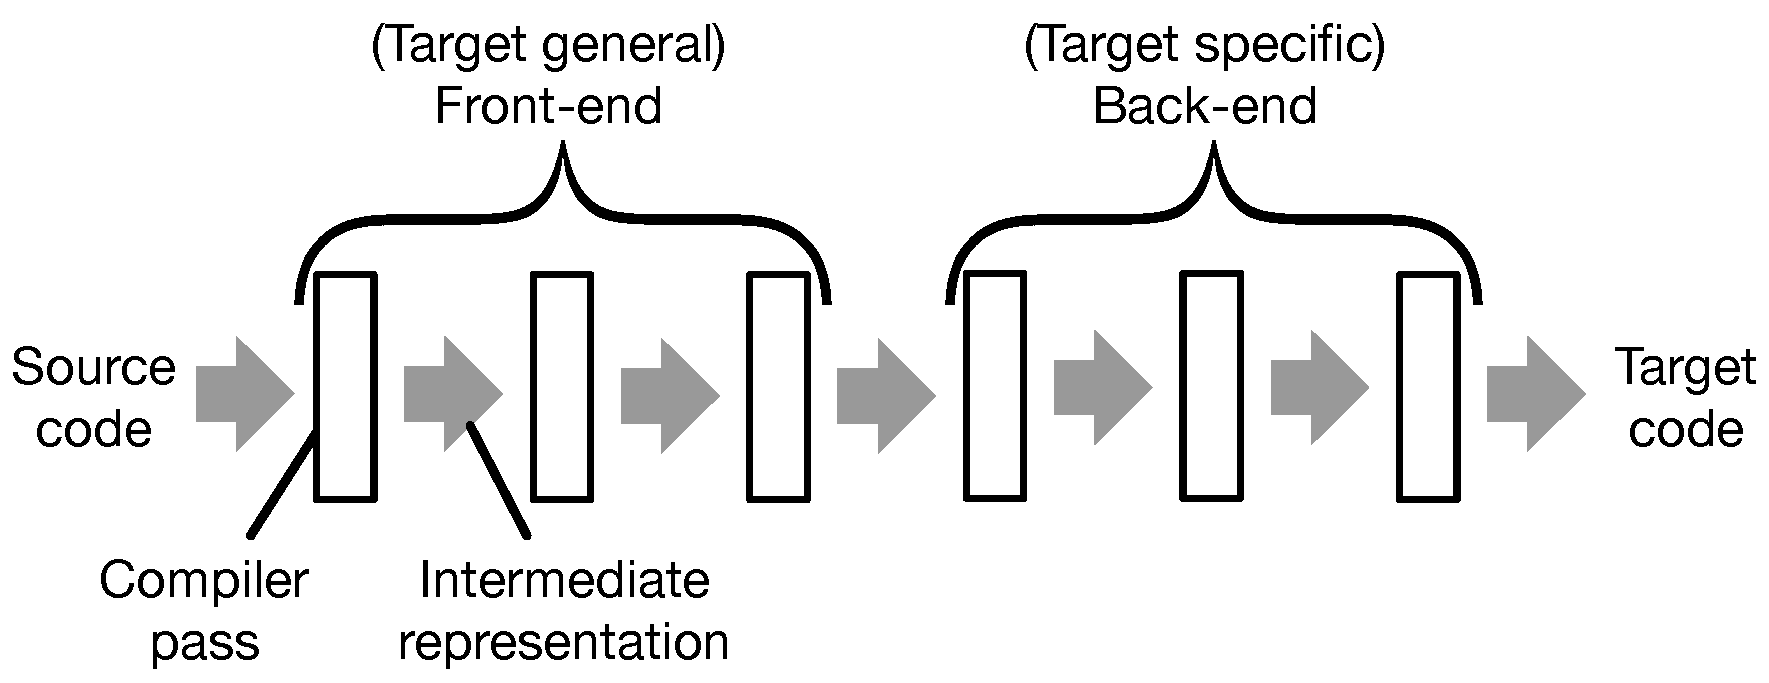
\includegraphics[width=0.9\textwidth]{compilation_overview.pdf}
\caption{P4's reference compiler~\cite{p4c} implements a typical
compilation pipeline: source code is transformed across several
passes, organised into front-end and back-end stages, to produce
target code. Its front-end stage consists of over 40 passes; this
diagram seeks to simplify.}
\label{fig:compilation:overview}
\end{subfigure}%
~
\begin{subfigure}[t]{0.5\textwidth}
\centering
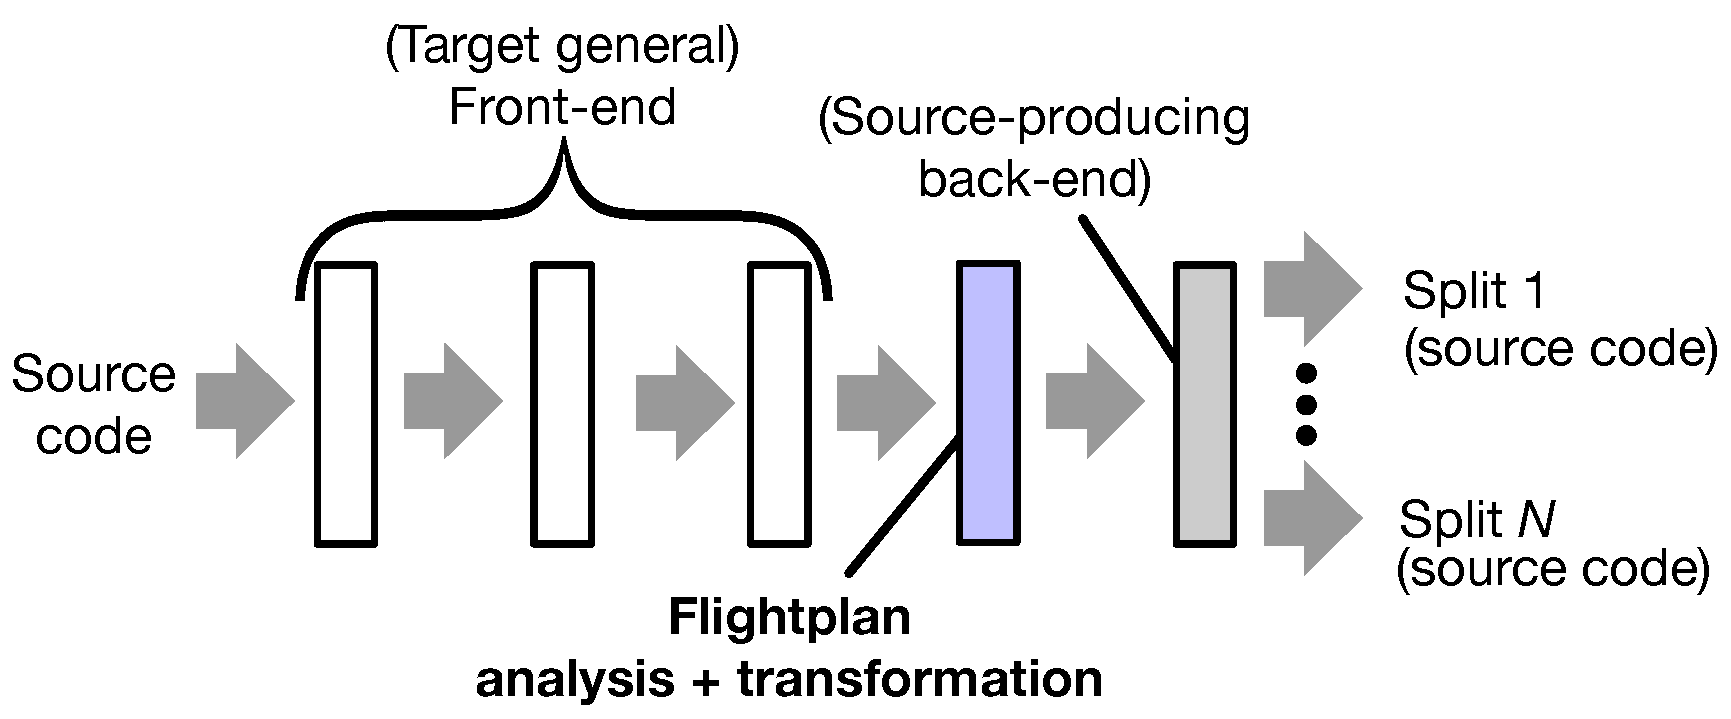
\includegraphics[width=0.9\textwidth]{compilation_flightplan.pdf}
\caption{Flightplan reuses completely the P4 reference compiler's
(target-general) front-end, and adds a pass to do Flightplan's
analysis and transformation into multiple splits. Each program split
can then be compiled for a specific target using that target's toolchain.}
\label{fig:compilation:flightplan}
\end{subfigure}
\caption{Flightplan's reuse and extension of the reference P4
compiler, for which different hardware targets' toolchains implement a
target-specific backend. Flightplan prefixes the normal P4
workflow with a code-splitting step, and does not require language or hardware changes.}
\end{figure*}

This increased network programmability heightens the importance of the question
of \emph{how} to program the network: how are distributed network elements
marshalled together to coherently implement a system wide application-servicing
policy?

The prevailing view is to have a \emph{network controller} play the role of a
network operating system~\cite{nox,pox}, maintaining a logically
centralised, global view of the network, and for the controller to mediate
between applications running above it, and dataplanes in the network.
Various studies have explored this
model~\cite{Voellmy:2013:MSS:2534169.2486030,voellmy2011nettle,onix},
yielding new insights, for example, on securely slicing a
large network~\cite{Casado:2006:SPA:1267336.1267346}, having multiple
cooperating controllers~\cite{Jin:2015:CCH:2789770.2789777}, operating networks
having elements that support varying degrees of
programmability~\cite{Jin:2015:TCL:2774993.2775013}, or scheduling changes to the
network while minimising disruption~\cite{Vissicchio:2017:SUH:3148626.3148643}.
This line of work followed the tipping point of more widespread programmability
made possible by OpenFlow~\cite{openflow-paper} and its industrial impact.

But this model was initially developed when switches' dataplanes were only
modestly programmable: affording only a limited vocabulary of actions, and
redirecting packets to the controller whenever non-trivial actions were needed. This limited programmability was one of
the constraints that P4 sought to relieve~\cite{p4}.
When considering these early dataplanes, the flexibility they offer seems less
like programmability, and more akin to improved \emph{configurability}, underscoring
OpenFlow's improvements over Ethane~\cite{ethane-sigcomm07}.

Thus as dataplanes become more programmable, a gap emerges between the
relatively simple network controller interface, and the programmatic capabilities of
productised~\cite{tofino,trident3} and
research~\cite{Sivaraman:2016:PTH:2934872.2934900,Chole:2017:DDP:3098822.3098823}
dataplanes.
This network-controller-based model can be improved to better match up
with the increased programmability made possible by P4 hardware
targets~\cite{Bosshart:2013:FMF:2534169.2486011}.

In this paper, we propose Flightplan, an approach that begins with
writing a single dataplane program that is then automatically split
into an arbitrary number of sub-programs that can be mapped into
different (and heterogeneous) dataplanes on the network.  The
composite behaviour of this distributed system is the same as the
original program; coordination and synchronisation code is
automatically generated. The programmer, or upstream programming tools
that generate the single dataplane program, are oblivious to the
logistical program transformation that turns it into a distributed
system.  This approach is possible using existing network hardware and
programming tools. Moreover, we retain the network controller's
important role in coordinating the network.

Flightplan effectively adds a generalisation of
RPC~\cite{Birrell:1984:IRP:2080.357392} support to P4, along with all the
automation this brings for stub generation.  Remote functions are extracted
from the original program, similar to
``exlining''~\cite{Vahid:1995:PEN:224270.224380}.
By combining the abilities of different dataplanes, we are able to realise
some ideas from active networking~\cite{Alexander:1997:AB:263109.263149},
in particular by using packets to activate continuations of computations along
dataplanes, rather than a more general design where packets carry explicit and
semi-arbitrary computations~\cite{Schwartz:2000:SPA:332799.332893}.

Figure~\ref{fig:overview} sketches our approach.
A key enabler of this approach is that P4, the foremost dataplane
domain-specific language, enjoys toolchain support to target diverse
hardware:
  ASIC~\cite{tofino},
  FPGA~\cite{sdnet,p4fpga,netcope},
  NPU~\cite{agilio},
  CPU~\cite{bmv2}.
These diverse targets' toolchains are based on P4's reference
compiler~\cite{p4c}, which we extend in our prototype
(Figure~\ref{fig:compilation:overview}).
P4's status as a common source language for diverse targets
simplifies our approach in comparison to post-hoc and
non-vendor-supported toolchains for targets that greatly exceed P4's
expressiveness, even if the same domain is being
targeted~\cite{203245}.

For this work we have developed a diverse suite of in-network
functions, including link-layer FEC, in-network cache, packet header
compression, and packet deduplication. We combine these as part of a
single large P4 use-case program, and demonstrate their interoperation
and distribution among a heterogeneous collection of hardware devices
running P4: CPU, FPGA, and ASIC.
The range of hardware targeted by P4 supports a common subset of P4
language features and differs others (such as the type and quantities
of state available to P4 programs, and the variety of external
functions that P4 programs may call).
\TODO{eval summary}

%Our goals are
%  flexibility when programming -- focus on the logic, not on topological details. automatically synthesise transfer of state.
%  programming support -- instrumentation, debugging, robustness
%  utilisation -- of equipment
%  performance -- load balancing, replicating programs
%    availability

\paragraph{Contributions}
\TODO{}
%\begin{enumerate}
%\item Flyto. Remote Program Segment. Linkage.
%\item Program transformation, separating logical segments, logical composition of programs.
%\item Coordination logic.
%\item Extern functions
%\end{enumerate}

\paragraph{Paper outline}
\TODO{}


\section{Automatic Dataplane Disaggregation}
\begin{figure}[t]
\centering
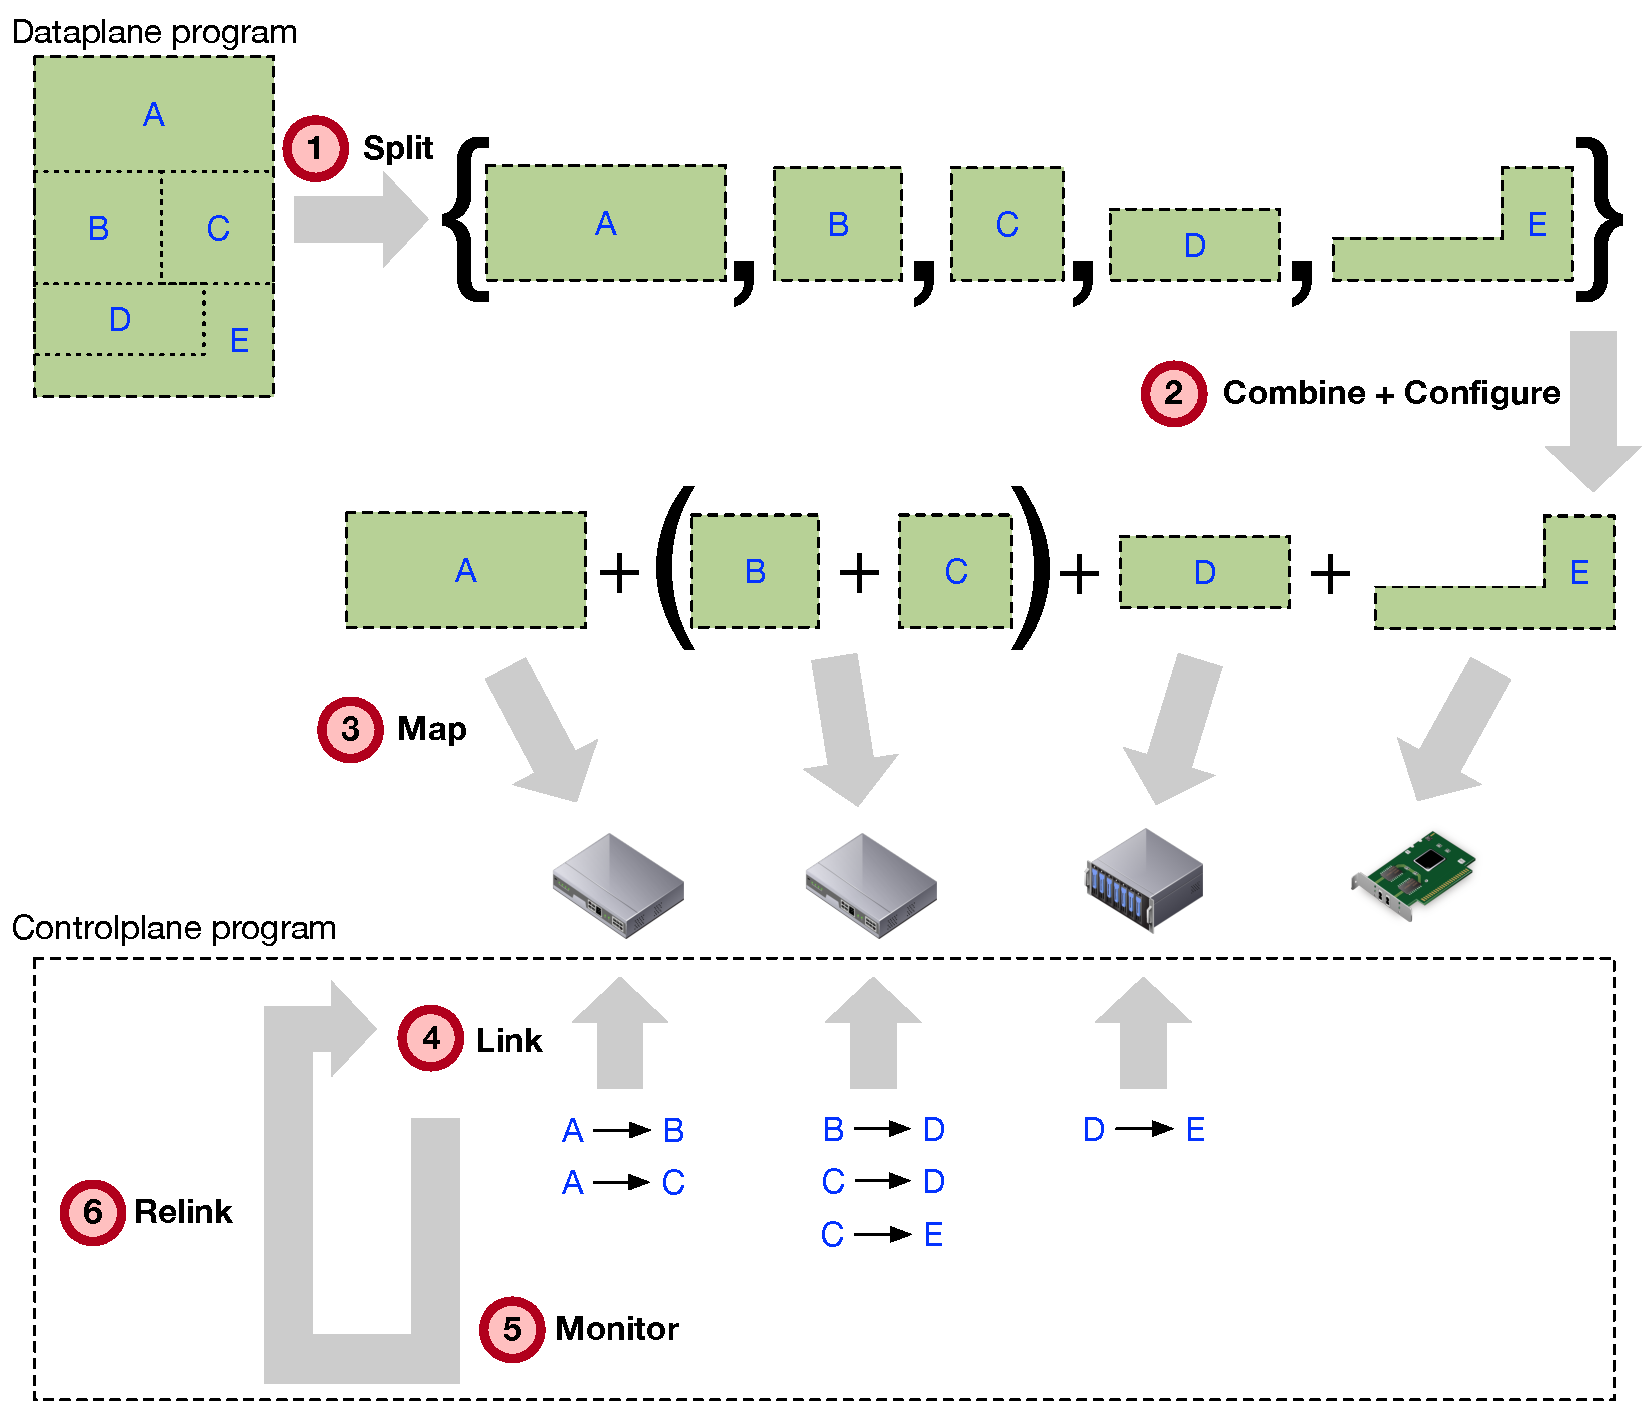
\includegraphics[width=0.5\textwidth]{workflow.pdf}
\caption{\label{fig:workflow}
\TODO{}  
In this illustration a program is split into 5 logical parts, {\sf\color{blue} A}-{\sf\color{blue} E}.
{\color{red}\ding{192}}~A program is annotated with logical delimiters, which Flightplan uses to split the program into complementary parts. Flightplan generates coordination and linkage code between these parts, which the network controller can configure at runtime.
{\color{red}\ding{193}}~Each split of the original program is mapped to a physical device. In this illustration,
 {\sf\color{blue} A} is a ToR switch,
 {\sf\color{blue} B} and {\sf\color{blue} C} are aggregation or core switches,
 {\sf\color{blue} D} is a CPU-run packet processor, and
 {\sf\color{blue} E} is an NPU.
{\color{red}\ding{194}}~The network controller can alter the program's linkage at runtime, to use different hardware targets, mitigate faults, or balance load.
}
\end{figure}

Combining the capabilities and resources of interconnected dataplanes
allows us to write more ambitious in-network programs.

\paragraph{Logical dataplane disaggregation}
%automatically split a program into a number of programs
\paragraph{Dataplane coordination}
%synthesising code between segments, to pass stuff along.
%  need \emph{transitive closure} of state
\paragraph{Physical mapping}
%Done online by the network controller
%failure handling
%load balancing
\paragraph{Heterogeneous targets}
%very important consideration
% trade-off in performance, host, and resources (memory + functions)
\paragraph{Language heterogeneity}
% different versions of P4
\paragraph{Cross-cutting concerns}
%Robustness
%Measuring
%can be transparently ``weaved'' into the program by our tool.
%~\cite{AOP}
\paragraph{Utilisation tuning}
%write once, run distributed
%the system will regenerate the interfaces for you
\paragraph{Performance tuning}
%Can move parts of the program between targets


\subsection{Workflow}
Figure~\ref{fig:workflow}.
\begin{enumerate}
\item Write program
\item Have spec of which externs are available
\item Logically split it
\item Install the splits
\item Configure the runtime
\item Run
\item Monitor + tune + hotswap + update
\end{enumerate}


\subsection{Runtime control}
Managed by the controller, which updates the flow tables in the targets.


\section{Use-case}
%API of functions
%Roster of resources?

\begin{figure}[t]
\centering
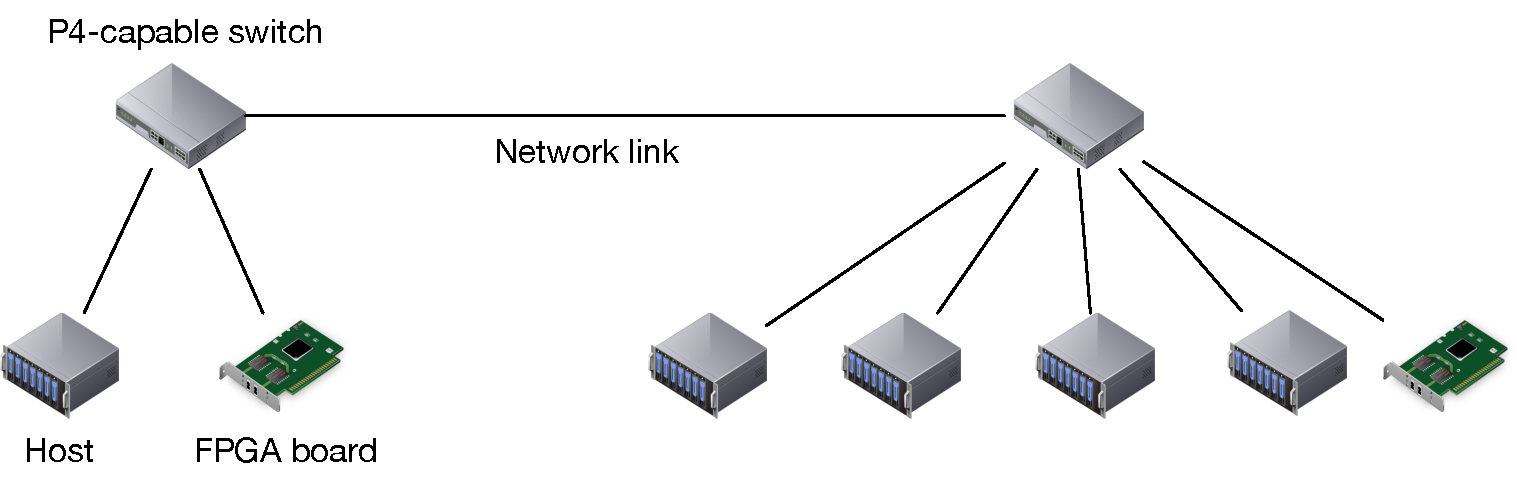
\includegraphics[width=0.5\textwidth]{eval_setup.pdf}
\caption{\label{fig:eval:setup}
\TODO{}  
}
\end{figure}


\begin{lstlisting}[caption=Program to be split.,
  label=listing:usecase,
  float=t]
#include "flightplan.h"
// Main control block
bla.apply();
flyto(PointAlpha);

\end{lstlisting}

We start with a dataplane program that involves various in-network functions,
as shown in Listing~\ref{listing:usecase}. In order to improve utilisation, or
indeed because of the resources we have available, we might want to run this
program across several dataplanes, such as in the heterogeneous network shown
in Figure~\ref{fig:eval:setup}.

\begin{figure}[t]
\centering
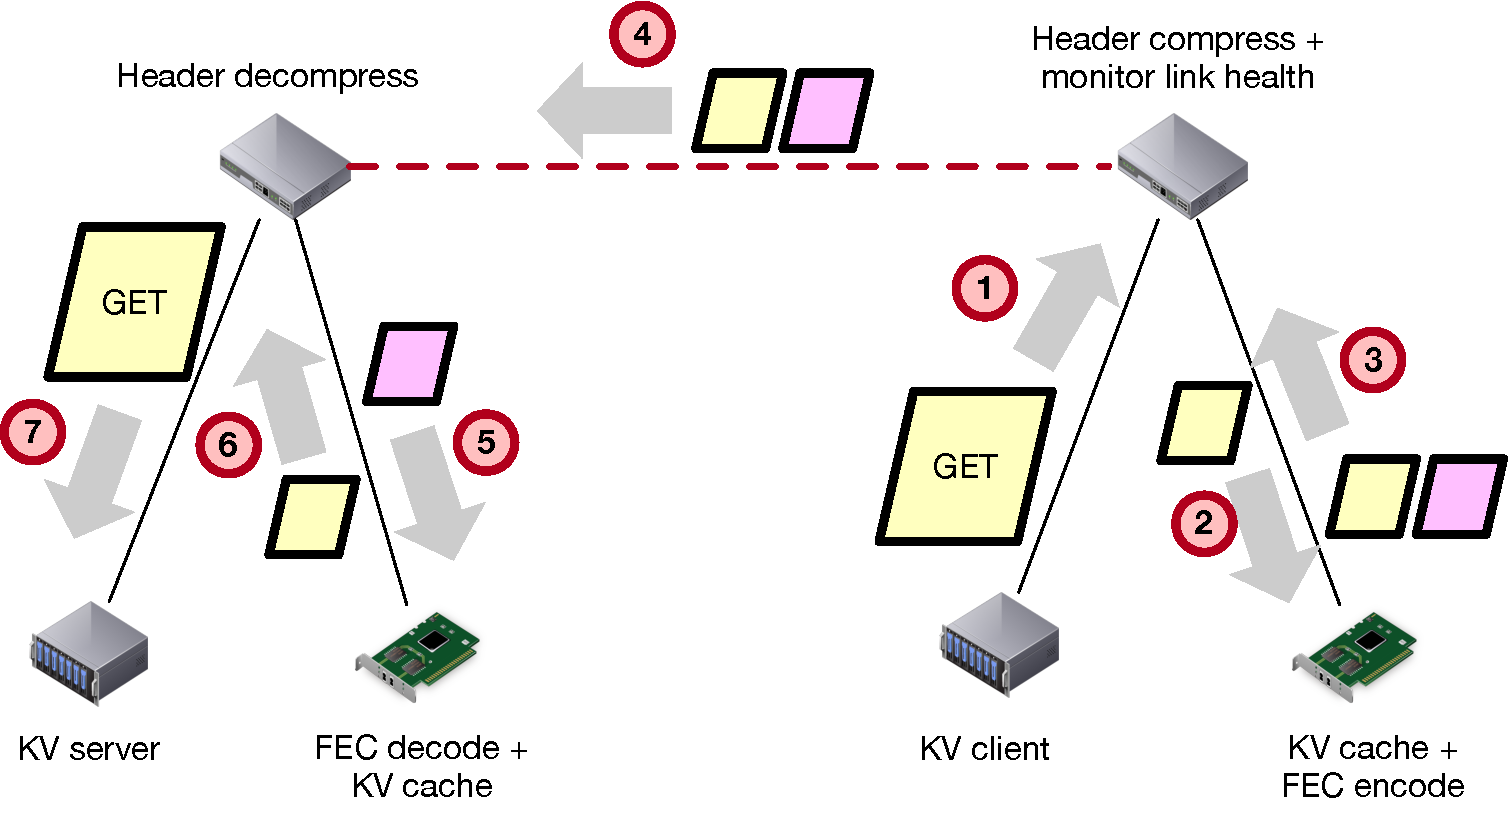
\includegraphics[width=0.5\textwidth]{scenario1.pdf}
\caption{\label{fig:usecase:scenario1}
\TODO{}  
}
\end{figure}


\section{In-network functions}
\subsection{Link-layer FEC}
\subsection{KV cache}
\subsection{Header compression}
\subsection{Packet deduplication}


\section{Flightplan}
Flightplan consists of three parts:
1)~declarations to be used in dataplane programs for splitting;
2)~an extension to the dataplane program compiler, carrying out analysis and
transformation;
3)~network controller for linking and monitoring the distributed dataplane program.

%Outputs: P4 programs, Controller API, and Compute/Resource mapping.

%For economy?
%Mapping part of the program into tables
%  finite functions
%
%
%turning synchronous into asynchronous

\subsection{Fault tolerance}
Failure-aware semantics, towards network exception handling~\cite{Karagiannis:2008:NEH:1402946.1402973}

\paragraph{Network failure}
\paragraph{Node failure}
\paragraph{Partial failure}
%dealing with network failure
%dealing with node failure -- loss of state, and loss of function (if cannot carry out some externs)
%error handling -- how to retry
%fault tolerance -- what if packets are erroneously duplicated?
%
%using redundancy
%  for more robustness, reliablity (having backup memory/functions)
%  for improved performance (having multiple workers)
%
%opportunities for debugging, can inspect state, and can rerun computation by replaying the calls.
%
%risk to security -- we assume a closed network.
%
%what if part of a program fails -- is the rest of the program ruined? can we resume/reattempt the computation?


\subsection{Transformation}
%  AST
%  vAST
%  paritioned AST
vAST, split-level topology, and ``stub'' interface generation.
Figure~\ref{fig:split-level-topology}.

\begin{figure}[t]
\centering
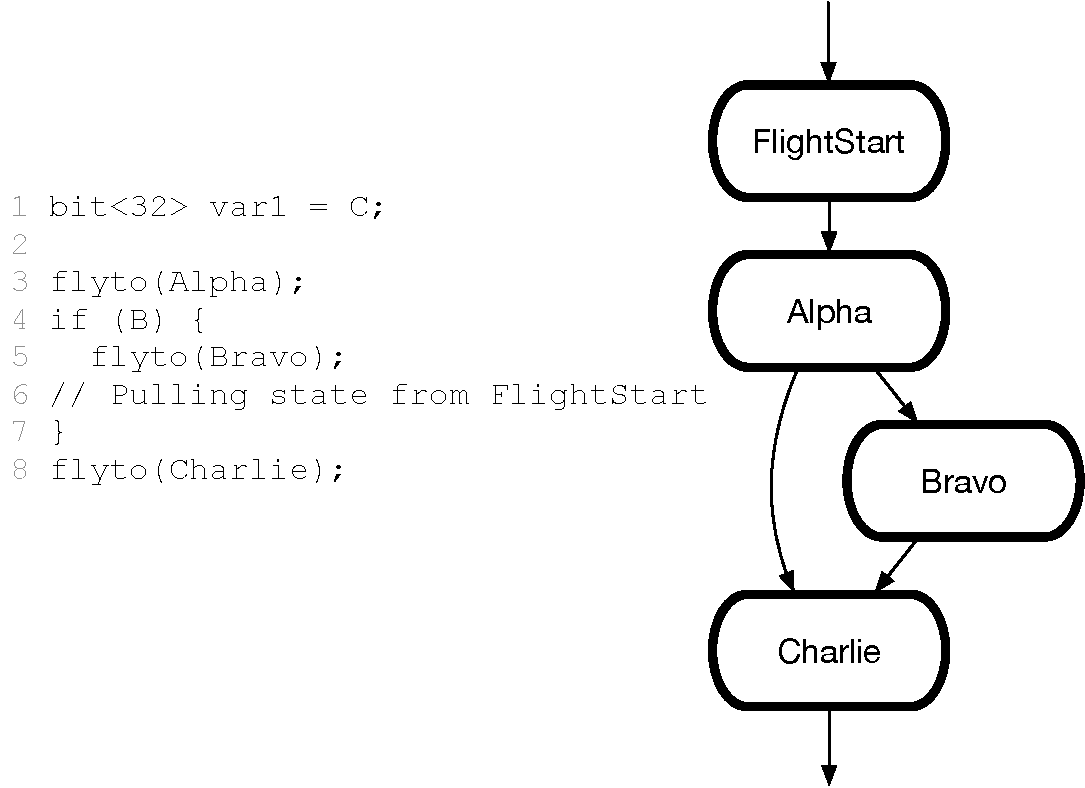
\includegraphics[width=0.5\textwidth]{split_level_topology.pdf}
\caption{\label{fig:split-level-topology}
\TODO{}  
}
\end{figure}

\subsection{Composition}
Generally possibly, as long as program's ``guard'' doesn't overlap. We can avoid the overlap since we generate the guard.


\section{Dataplane program portability}
Comparing SDNet and BMv2 extern interface,
and Tofino (if not NDA'd).
\verb+#ifdef+-based platform targeting.


\subsection{Setup}
Control programs running on the network controller

Target-feature usage
Using memory in different backends, having magic externs for some uses — e.g., memory (read/write/atomic increment).
 Inspired by how emulate instructions across architectures.

Complexity of programs


\section{Evaluation}
Setup, topology.

Platforms:
Tofino,
x86 CPU,
FPGA,
%Netronome.

\TODO{Goals}

\subsection{Distributed performance}
Granularity of splitting. Local vs remote externs.

Overhead: monolithic vs distributed FEC externs.

\subsection{Flexibility}
Distribution vs load vs proximity
Availability

\subsection{Utilisation}
Utilisation vs performance

Latency

Throughput

Disaggregation strategies


\section{Related work}
%Domino + RW
%
%Stateful network functions
%
%\cite{Jeyakumar:2014:MLM:2740070.2626292}


\section{Conclusion}


\section{Acknowledgments}
Anirudh Chelluri and Lei Shi.
Perspecta Labs.
Funders.

%\section{Availability}
%
%It's great when this section says that MyWonderfulApp is free software, 
%available via anonymous FTP from
%
%\begin{center}
%{\tt ftp.site.dom/pub/myname/Wonderful}\\
%\end{center}
%
%Also, it's even greater when you can write that information is also 
%available on the Wonderful homepage at 
%
%\begin{center}
%{\tt http://www.site.dom/\~{}myname/SWIG}
%\end{center}
%
%Now we get serious and fill in those references.  Remember you will
%have to run latex twice on the document in order to resolve those
%cite tags you met earlier.  This is where they get resolved.
%We've preserved some real ones in addition to the template-speak.
%After the bibliography you are DONE.

{\footnotesize \bibliographystyle{acm}
\bibliography{paper}}

\theendnotes

\end{document}
